\chapter{Related work}

\pagestyle{fancy}

\label{relatedWork}

At the moment, the biggest names on the market, when talking about world generation, are \textit{Terragen}\cite{terragen} and \textit{World Machine}\cite{worldMachine}. There are some new projects that start to make a name for themselves, such as \textit{GAEA}\cite{gaea}, but they are yet to reach the maturity level of the other ones. \textit{World Machine} is based on powerful fractal noise algorithms that can produce both realistic and highly-stylized terrain. It offers a wide range of settings and parameters that can be tweaked, in order to obtain the desired results. A graph-based interface is also implemented, offering a more graphic representation of the available settings, thus improving the workflow of many users. Features like rivers and lakes are one click away, and erosion simulations such as \textit{flow based erosion} and \textit{thermal erosion} are highly abstractized, so that anyone can make use of them without much knowledge of how things work "under the hood". Advanced texturing options are also available, with detailed filters affecting even the \textit{areas of erosion} and \textit{talus depositions}. From generation of snow-covered mountains, surrounded with dense forests, to barren deserts and even cosmic vistas, this type of software offers an unprecedented level of artistic freedom, with some of the scenes created within them being simply breathtaking (see Figure \ref{fig:terragen}).\\

There are numerous smaller projects available at the moment, many of them even being free, since they are developed by individual developers that are just having fun coding. Besides standalone software, there are also a lot of tools and extensions for existing computer graphics software, especially game engines, such as \textit{Unreal Engine 4} and \textit{Unity Engine}. If in a hurry, one can use these community-created assets to speed up their game's development process. Some examples of smaller plugins and frameworks are \textit{Proceduraltoolkit}, \textit{Sorcar} and \textit{Tree Gen}. \textit{Proceduraltoolkit} is an all-purpose package, able to create everything from chair and building models, to "low-poly" style terrain and mazes. \textit{Tree Gen} is a \textit{Blender} plugin, designed to exclusively generate all kinds of trees, and is actually part of a student's undergraduate dissertation\cite{hewitt2017procedural}.\\

When talking about games, it is impossible not to mention \textit{Minecraft}, which we already covered previously. This video game alone has generated nearly \$500 million since 2014, when \textit{Mojang} studio was bought by \textit{Microsoft}, for \$2.5 billion\cite{minecraftRevenue}, proving that a project that is not particularly impressive graphics-wise, can offer so much content through the powerful concept of procedural generation. Another classic example is \textit{Spore}, developed by \textit{Maxis} and published in 2008. Similar in some ways to \textit{No Man's Sky}, \textit{Spore} uses deterministic algorithms to generate 3D creatures, terrain, planets and even spaceships and galaxies. At launch, it was a "breath of fresh air", because previously, games that were based on this type of algorithms were more obscure and not that popular.

\begin{figure}[htp]
    \centering
    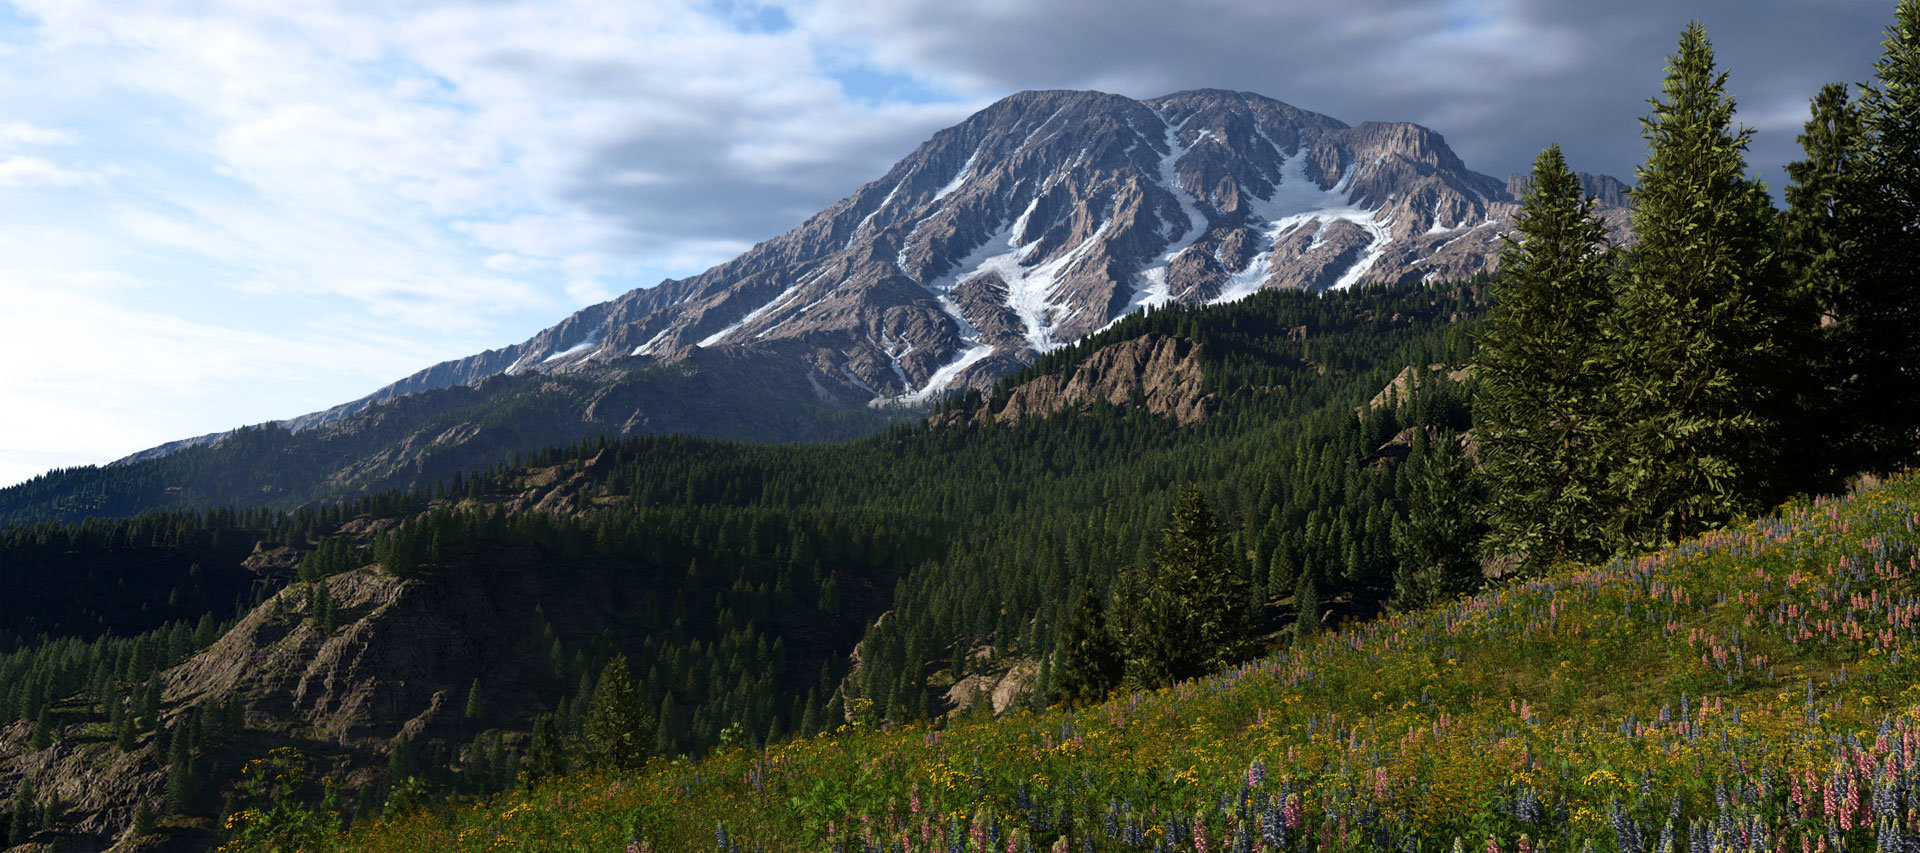
\includegraphics[width = 16cm]{figures/terragen.jpg}
    \caption{A mountain scene created and rendered with \textit{Terragen 4}.}
    \cite{terragen}
    \label{fig:terragen}
\end{figure}